\section{General outline of the purse}
All of the \textit{Smart Cards} applications are split out in two
parties$:$ an extern application to the card (called terminal) and an
internal one (called applet). The electronic purse is a
\textsc{JavaCard} application which intends to provide to card holder,
the ability to execute bank operations. This application is loaded in
the smart card as an applet. The figure~\ref{fig-cas-pur} shows the
general outline of this application.




\begin{center}
\begin{figure}[hbt]
\rule{\linewidth}{0.3mm}
\\[2.5ex]
\centering
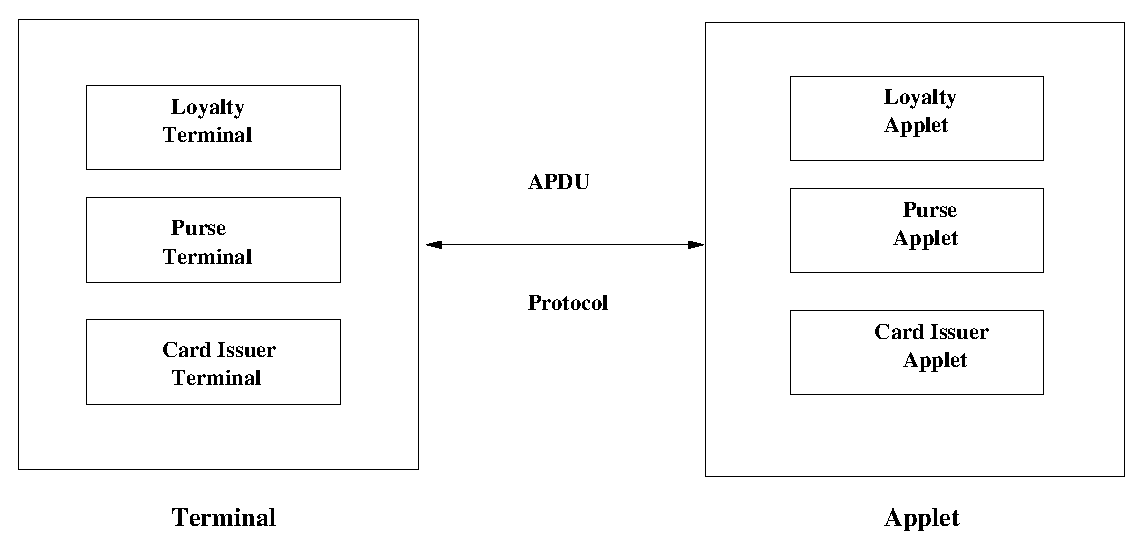
\epsfig{file=figures/javacard.eps, width=11cm, clip=}
\caption{Outline of the purse}
\label{fig-cas-pur}
\rule{\linewidth}{0.3mm}
\end{figure}
\end{center}




The  \texttt{CardIssuer} applet has personal information of the card
holder and contains the pine code of the card. The \texttt{Purse}
applet carries out the \textit{credit} and \textit{debit}
operations. This applet allows the card holder also to change its
currency type. Apart from that, this applet has several mechanisms
which do not allow to execute some commands when the applet is not
found in a suitable state. The applet \texttt{Loyalty} handle a
counter which is increased when any purchase is carried out, and when
a debit operation is failed, the application will see the available
money in this counter.


\paragraph{The \textit{debit} operation.}
This operation allow us to carry out a debit transaction. Thus, if
severals transaction are done in the same session, it is possible that 
the card user presents once his pine code for transaction lesser than
\texttt{maxDebitWithOutPIN}. This variable represents the biggest
quantity that a client may credit without present his pine code. For
security reasons, the card holder can do at most
\texttt{maxTransactionWithoutPIN} transactions in a same session. 


\paragraph{The \textit{credit} operation.} When the purse is empty, the 
card holder can be do an debit operation. In this case, the terminal
sends the bank a request asking for any credit permission. If the card 
holder has some one the bank will send to the terminal a certificate of 
this permission. 



\paragraph{The \textit{Currency} operation.} The balance is related to a
currency. When the card holder travels he has the possibility to
change the currency. In this case, the terminal request to the bank a
new exchange rate and a certificate. The purse verify than the bank is 
really the expected bank and it validates the exchange rate. After
changing the balance value, the purse must modify all the variables
that are related to the currency. \\

When a currency change occurs, the purse sends to the loyalties a
\textit{changeCurrency} warning. It is expected than each loyalty
request to the purse all logged transaction.  Then the purse may erase 
the log transaction file. The purse can be associated to different
loyalties and it must differentiate them when the purse is sending
their logged transactions. \\
